% !Mode:: "TeX:UTF-8"

\chapter[受空气阻力的弹道迭代计算]{受空气阻力的弹道迭代计算}[Harbin Institute of Technology Postgraduate Dissertation Writing Specifications]



\section{空气阻力系数求解}[Content specification]
其中因为在y⽅向分速度较⼩,可以忽略不计,因此只考虑x⽅向的空⽓阻⼒。空气阻力计算公式如下:
\begin{gather}
    F = kv^2 =  \frac{1}{2} CS \rho  v^2
\end{gather}

\par

其中$\rho$为空气密度,一般取$1.293kg/m^3$,S为球截面积,$v$为球体速度,C为阻力系数,与雷诺数$R_e$有关系,关系如图\ref{空气阻力系数与雷诺数关系}所示。

\begin{figure}[H]
    \centering
    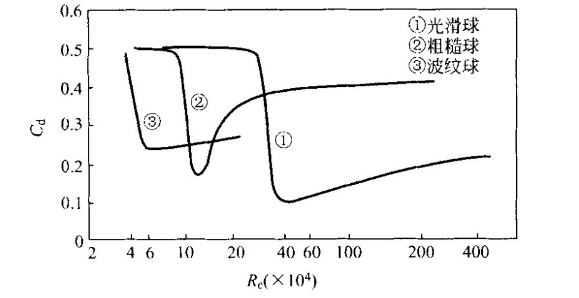
\includegraphics[width=.8\textwidth]{leinuo.png} 
    \caption{雷诺数} 
    \label{空气阻力系数与雷诺数关系}
\end{figure}

\par 

雷诺数计算公式如下:
\begin{gather}
    R_e = \frac{\rho v D}{\eta}
\end{gather}

其中$\rho$为空气密度,一般取$1.293kg/m^3$,D为物体直径,$v$为球体速度,$\eta$为空气粘滞系数,通常取$1.983\times10^{-5}pa\cdot s$


\section{弹道迭代计算}
\begin{figure}[H]
    \centering
    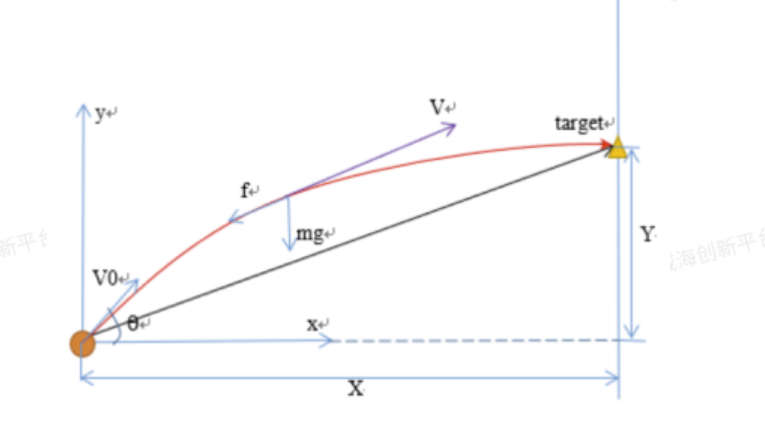
\includegraphics[width=.8\textwidth]{trajectory.png} 
    \caption{弹丸受力分析图} 
    \label{弹丸受力分析图}
\end{figure}

如上所述,我们只考虑水平方向的空气阻力。弹丸的动力学微分方程如下:
\begin{gather}
    m \frac{dv_x}{dt} = -k v_x^2 \\
    m \frac{dv_y}{dt} = -mg
\end{gather} 

采用分离变量法求解微分方程,可得:
\begin{gather}
    v_y = v_{y0}-gt \\
    v_x = \frac{m v_{x0}}{m+kv_{x0}t}
\end{gather}

消去时间变量$t$,可推导出如下动力学公式:
\begin{gather}
\frac{gm^2\lambda^2 tan^2(\theta)}{2k^2v^2}-\frac{\lambda m tan^2(\theta)}{k}+\frac{gm^2\lambda^2}{2k^2v^2}+y = 0
\end{gather}

其中:
\begin{gather}
    \lambda = e^{\frac{kx}{m}-1}
\end{gather}

代入目标位置即可求得子弹飞行时间$t$和云台姿态角$pitch$。\par
然而待击打的物体是在运动的,若是直接拿观测坐标计算弹道,则弹丸在打过去的时候,
目标已经离开原来位置,出现击打滞后现象。但是,考虑目标运动的弹道解算想要求解析解几乎是不可能的,因此我们退而求其次,通过数值
迭代的方式求数值解。基本思路为:
\begin{enumerate}
    \item 按照初始位置矢量计算弹道,解算飞行时间$t_0$。
    \item 根据此飞行时间计算目标位移量$\Delta \vec{x_0}$。
    \item 根据目标位移量计算新的位置矢量$\vec{x_1}$。
    \item 跳转至1过程。
\end{enumerate}

如图\ref{迭代计算过程}所示:

\begin{figure}[H]
    \centering
    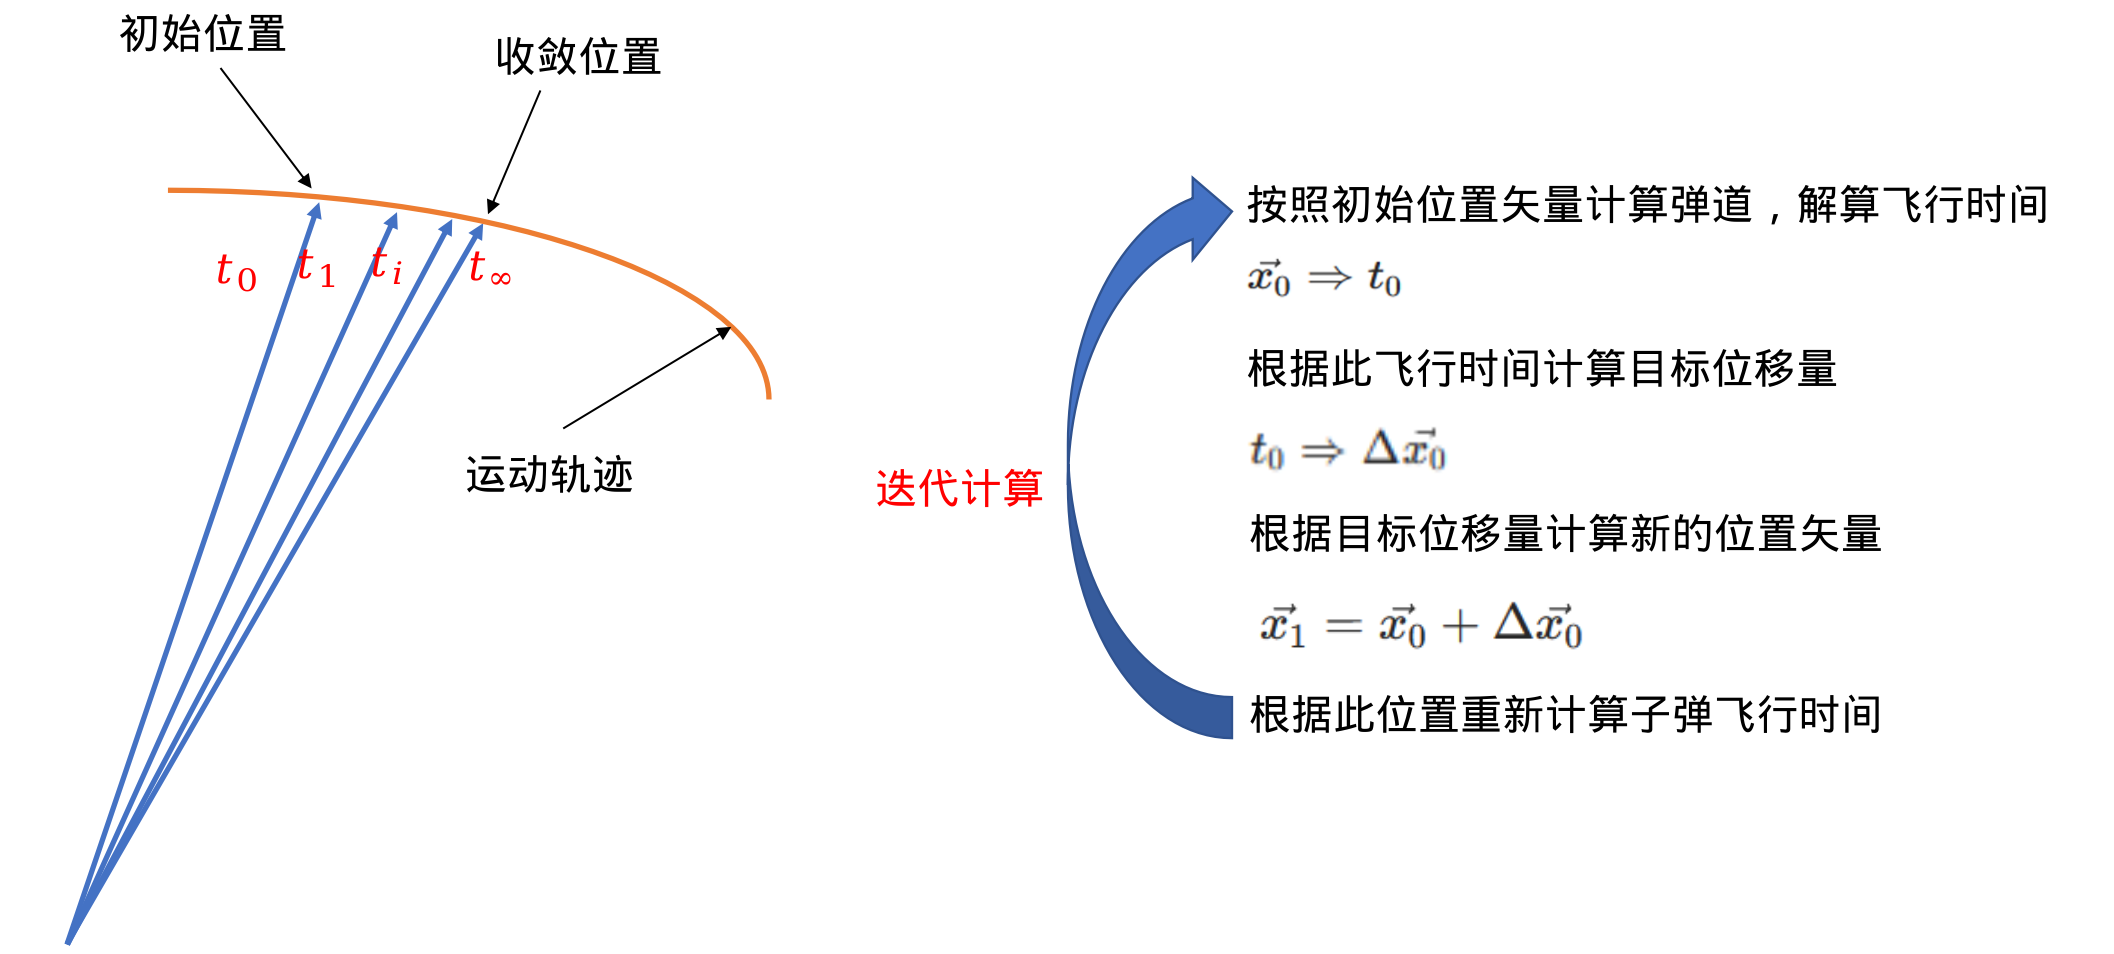
\includegraphics[width=.8\textwidth]{iter.png} 
    \caption{迭代计算过程} 
    \label{迭代计算过程}
\end{figure}